\section{Results}

\end{multicols}
	
\begin{table}[H]
\centering
\begin{tabular}{llcc}
\toprule
Model & Technique & (Macro) F1 & Balanced Acc. \\
\midrule
\multicolumn{4}{l}{\textbf{Traditional ML}} \\
Decision Tree & -- & 0.675 & 0.685 \\
Random Forest & -- & 0.720 & 0.719 \\
Gradient Boosting & -- & 0.722 & 0.718 \\
Support Vector Machine & -- & 0.652 & 0.635 \\
$k$-Nearest Neighbors & -- & 0.601 & 0.595 \\
MLP Classifier & -- & 0.678 & 0.676 \\
ELM Classifier & -- & 0.645 & 0.630 \\
\addlinespace
\multicolumn{4}{l}{\textbf{LLMs}} \\
Qwen-2.5-3B & 0-shot & 0.218 & 0.297 \\
Qwen-2.5-3B & 1-shot & 0.387 & 0.562 \\
Qwen-2.5-3B & 5-shot & 0.306 & 0.377 \\
LLaMA-3-8B & 0-shot & 0.280 & 0.341 \\
LLaMA-3-8B & 1-shot & 0.392 & 0.509 \\
LLaMA-3-8B & 5-shot & 0.481 & 0.494 \\
\bottomrule
\end{tabular}
\caption{Summary of traditional ML and LLM performance on the test set (Macro F1 and Balanced Accuracy).}
\label{tab:results-summary}
\end{table}
	
\begin{figure}[H]
\centering
	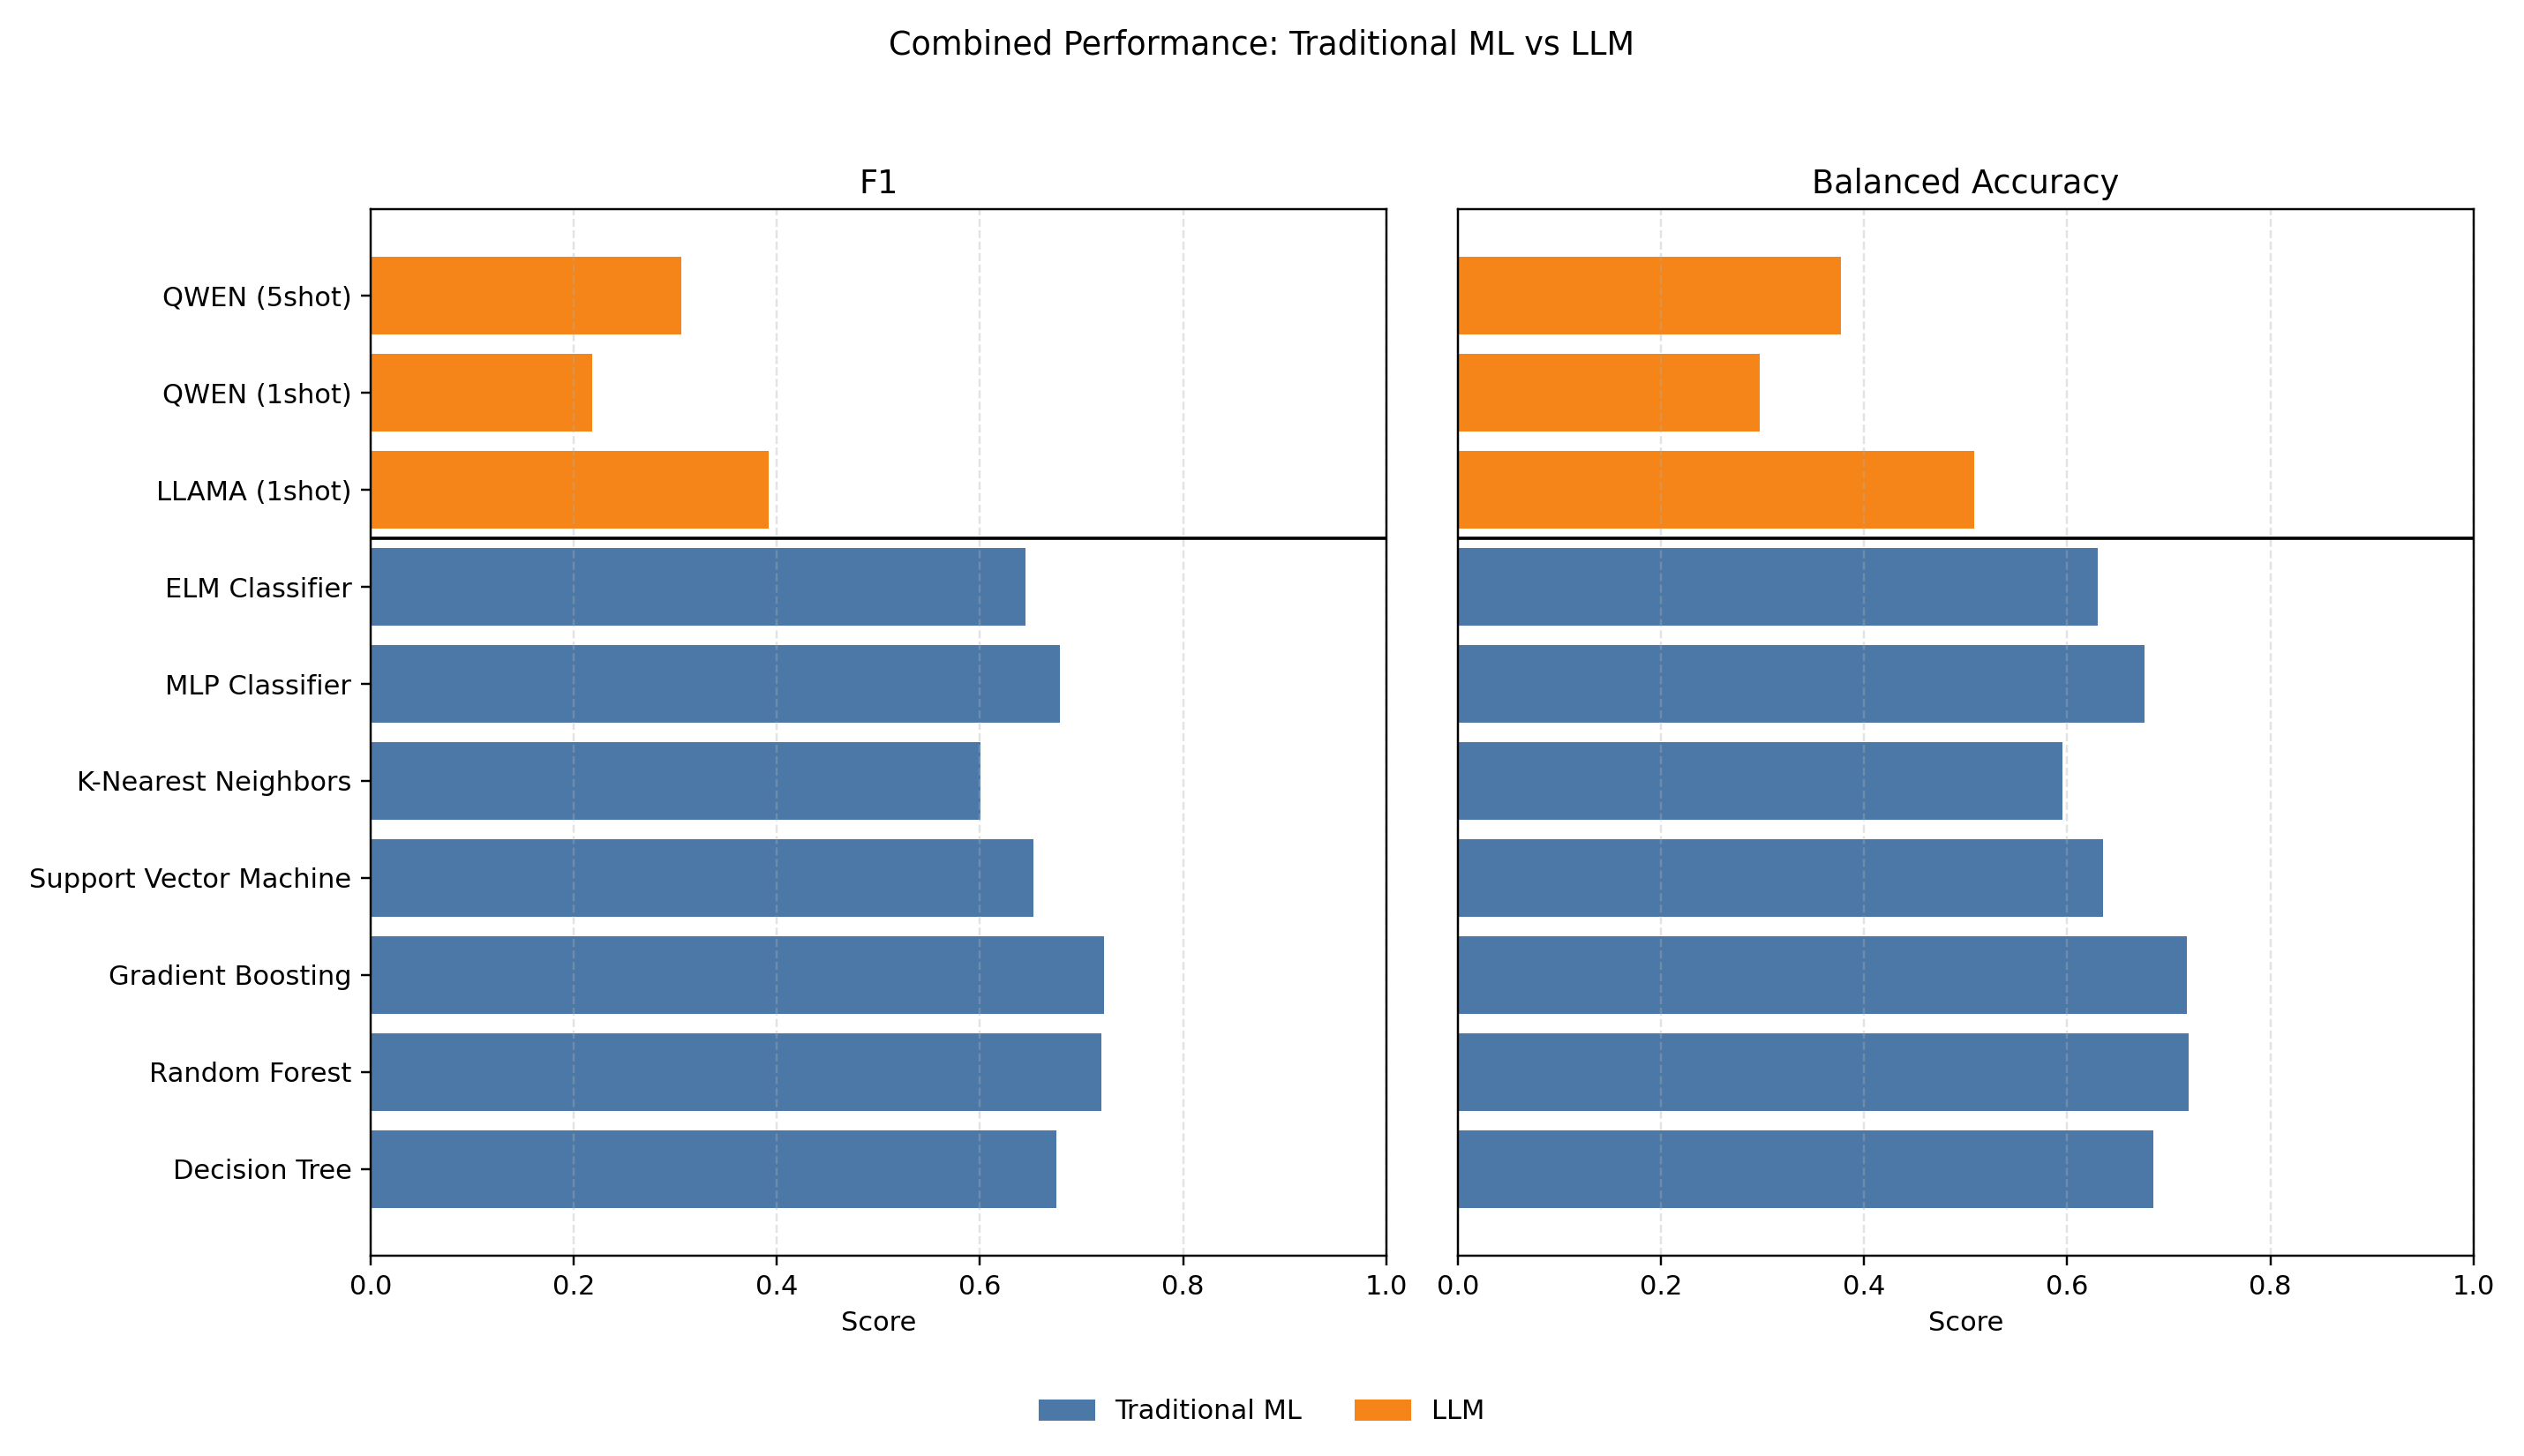
\includegraphics[width=\textwidth]{code/plots/combined_tradml_llm_performance.png}
	\caption{Combined performance comparison of traditional machine learning models and large language models using F1 and Balanced Accuracy.}
    \label{fig:combined-performance}
\end{figure}

\begin{figure}[H]
\centering
	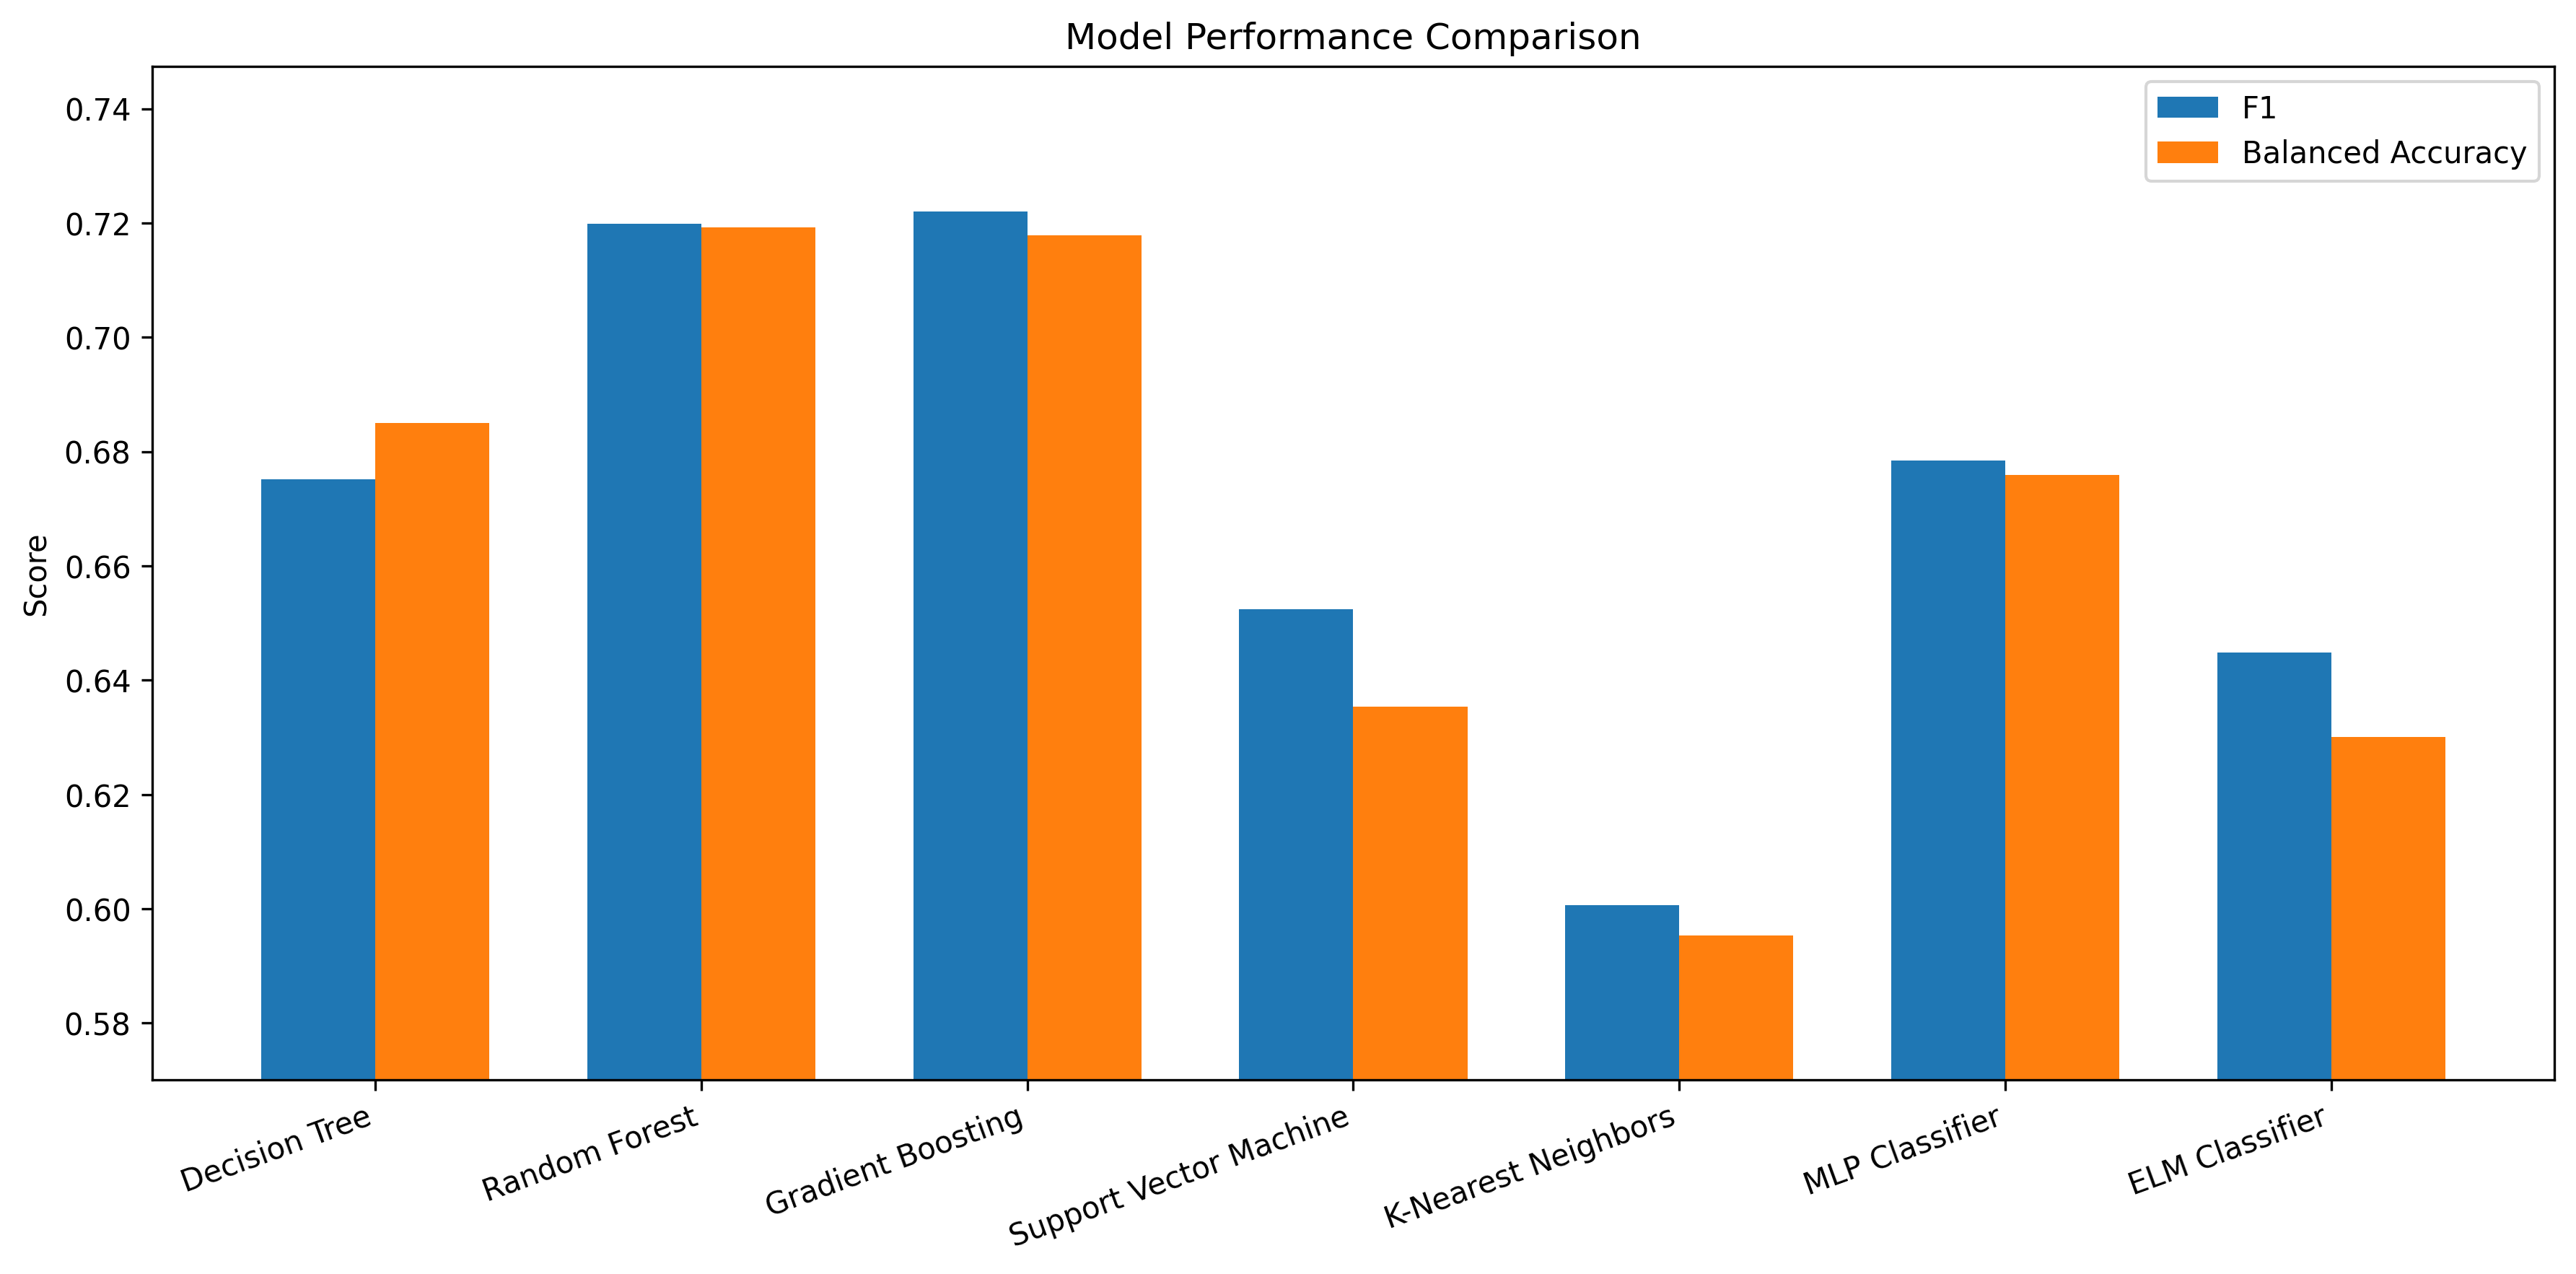
\includegraphics[width=\textwidth]{code/plots/model_performance_py.png}
	\caption{Test-set performance comparison of traditional predictive models using Macro F1 and Balanced Accuracy.}
    \label{fig:tradml-performance}
\end{figure}

\begin{multicols}{2}

\subsection{Traditional Predictive Models}
Various traditional model architectures are implemented. The evaluated models are Random Forest, Decision Tree, Support Vector Machine, Gradient Boosting, $k$-Nearest Neighbors, Extreme Learning Machine, and Multilayer Perceptron. The performance of each model is measured using plain accuracy, balanced accuracy, and F1 score. The accuracy of a model can be calculated as
\[
	\frac{\text{True Positive} + \text{True Negative}}{\text{Total Predictions}}.
\]
It is an intuitive measure of how correct the model predictions are, but falls short when the given dataset is imbalanced. To mitigate this issue, the balanced accuracy is preferred:
\[
	\frac{\text{Sensitivity} + \text{Specificity}}{2}.
\]
In addition, the F1-score is also utilized, calculated as the harmonic mean of precision and recall:
\[
	\frac{2 \times \text{Precision} \times \text{Recall}}{\text{Precision} + \text{Recall}}.
\]
As shown in Fig.~\ref{fig:tradml-performance}, the model performance plot summarizes the comparative results across all evaluated traditional predictive models. Ensemble methods remain the top performers, with Gradient Boosting and Random Forest achieving the highest F1 scores of 0.722 and 0.720, respectively. Support Vector Machine and Extreme Learning Machine also show competitive performance, while $k$-Nearest Neighbors has the lowest F1 among the traditional models at 0.601. These results are consistent with existing literature that highlights the effectiveness of ensemble methods in classification tasks, particularly in educational contexts where complex interactions between features are common.

\subsection{Large Language Models}
\begin{figure}[H]
	\centering
	\begin{minipage}{0.5\textwidth}
		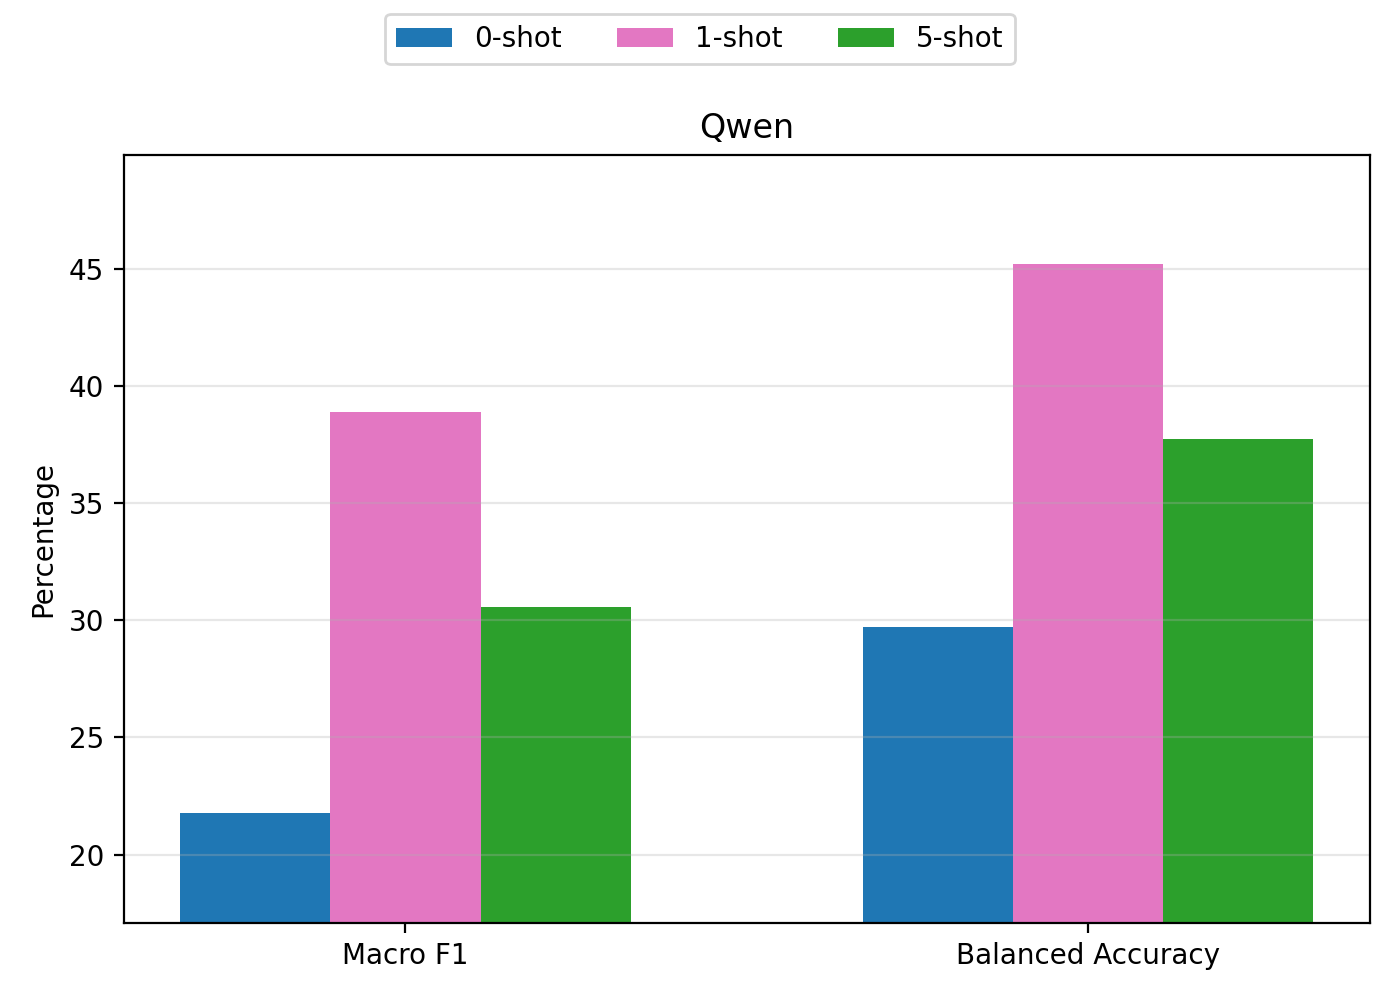
\includegraphics[width=\textwidth]{code/plots/qwen_metric_technique_comparison.png}
	\end{minipage}
	\begin{minipage}{0.5\textwidth}
		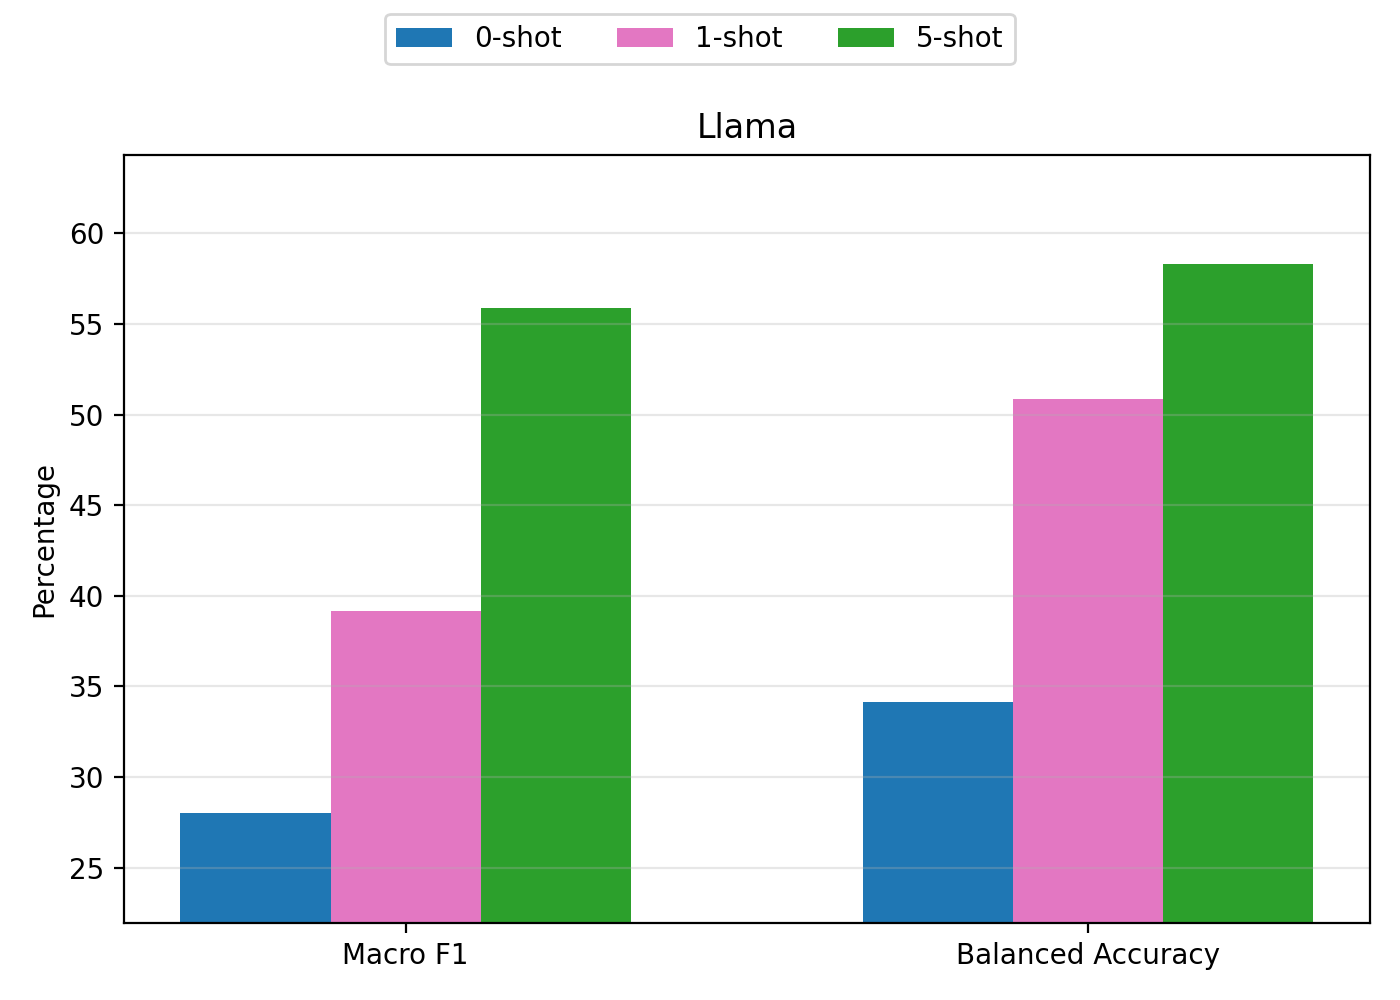
\includegraphics[width=\textwidth]{code/plots/llama_metric_technique_comparison.png}
	\end{minipage}
	\caption{Prompting-technique comparison for Qwen-2.5-3B (left) and LLaMA-3-8B (right), using Macro F1 and Balanced Accuracy.}
    \label{fig:llm-prompting}
\end{figure}
We report Macro F1 for LLMs. Macro F1 treats each class as equally important by averaging the per-class F1 scores. This is particularly useful in our case, where the dataset is imbalanced, and we want to ensure that performance on minority classes (e.g., at-risk students) is not overshadowed by performance on majority classes (e.g., passing students). As shown in Fig.~\ref{fig:llm-prompting}, the best-performing LLM configuration is LLaMA-3-8B with 5-shot prompting, which achieves a Macro F1 of 0.481 and a balanced accuracy of 0.494. Qwen-2.5-3B performs best with 1-shot prompting (Macro F1 = 0.387; balanced accuracy = 0.562). Overall, Macro F1 values range from 0.218 to 0.481 and balanced accuracies range from 0.297 to 0.562.

Even the best-performing LLM configuration (LLaMA-3-8B with 5-shot prompting) achieves a Macro F1 of only 0.481, which is lower than the lowest-scoring traditional model ($k$-NN with a Macro F1 of 0.601). This suggests that the bottleneck is not model capacity---LLaMA-3-8B has 8 billion parameters compared to $k$-NN's zero learned parameters---but rather the mismatch between the LLM pretraining distribution (natural language) and the input modality (serialized numerical feature vectors).

This gap also contextualizes the practical implications for HEIs: at current scales, deploying general-purpose LLMs for student outcome classification without fine-tuning would produce predictions no better than a majority-class baseline, rendering them unsuitable for early-warning systems where per-class sensitivity is critical.